\asection{Graph Basics}
\label{Graph Basics}


\setlistdepth{9}

\newlist{myEnumerate}{enumerate}{9}
\setlist[myEnumerate,1]{label=(\arabic*)}

\label{Graph Overview}
A Graph in Mathematics and Computer Science is a pair G = (V, E),  where V is the set of vertices and E is the set of edges, formed by pairs of vertices with each other. Figure 1 demonstrates the structural 
attributes of a simple graph graph.

\begin{figure}[H]
  \begin{center}
      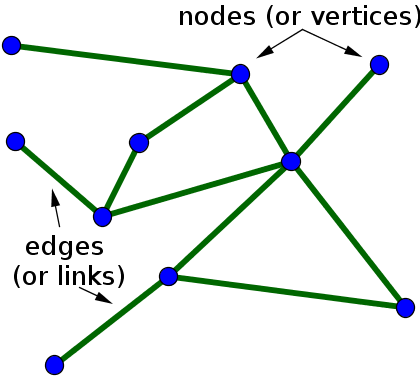
\includegraphics[width=0.65\textwidth]{graph.PNG}
  \end{center}    
  \caption{Representation of a graph}
\end{figure}

Graphs can either directed or they can undirected. This means that the edges in the graph could have an abscence of direction as in the figure above, or they could have a direction showing from which
vertice the edge is coming from, and to which vertice the edge is going to. The figure below demonstrates a directed graph, commonly known as a digraph. This characteristic is demonstrated by the edge 1, 
that goes from node a to node b, and also by edges 3 that goes from node c to node a. Note that the undirected graph mentioned above is commonly referred to as a bigraph because the direction
of its edges  could be percieved as to goiing in both direction as it is not specifed.\newline\newline
In this paper, the focus is primarily on directed graphs, and they shall be referred to as digraphs from here onward.

\subsection{Digraph}
A Digraph in mathematics is defined as is a pair of vertices and edges (V,E) that are disjoint, and their repective mappings that comprise of two components, namely the initial vertix and 
terminal vertice of each edge i.e. each edge has a initial vertix: Ei->Vi and a terminal vertix Vj->Ej for some vertices Vi,Vj in V and edges Ei,Ej in E[7], refer to the figure above.

\subsection{Graph representation}
Graphs are represented in a variaty of ways, from adjacency lists, incident matrices and adjacency matrices. The algorithms that are studied in this paper make us of adjacency matrices and
adjacency list representations of graphs. 

\subsubsection{Adjacency matrices}
An adjacency matrices is a nxn matrix A, with A(i,j) = 1 iff(i,j) ∈ E[9]. This means that wherever there is an edge in the graph, it is denoted by a 1 in the matrix, places in the matrix A where there is an absence of an edge E are denoted by 0.\\\\
Figure 4 depicts the association between a graph and its adjacency matrix.

\subsubsection{Adjacency list}
An Adjacency list is vertices of a graph, of which each vertice is connected to the list. The vertices in an adjacency list point to their own list of edges that they are connected to(i.e. the list contains the edges that connectect them to other vertices).
Figure 4 depicts an example of an adjacency list.

\subsection{Supergraphs and subgraphs}
Let GA be be graph define as follows GA = (VA,EB) and let GB be another graph that is defined as follows GB = (VB,EB) where VA,VB are sets of vertices and EA,EB are sets of edges.
In graph theory, a graph GA is said to be a subgraph of graph GB, and graph GB is said to be a supergraph of graph GA if all the vertices and edges that are in graph GA are also in graph
GB, that is [3]\newline\newline

\begin{myEnumerate}
  \item VA <= VB, and
  \item Every edge of GA is also an edge in GB.
\end{myEnumerate}